\documentclass[11 pt]{article}
\usepackage[a4paper, total={6in, 8in}]{geometry}
\usepackage{float}
\usepackage{multirow}    % to add multirow cells in tables
\usepackage{indentfirst} %to automatically intent the first paragrap of each sections
\usepackage{amsmath}		%math packages
\usepackage{mathtools}
\usepackage{amssymb}
\usepackage{graphicx}	%Required for inserting images
\usepackage{fontenc}
\usepackage[colorlinks=true,linkcolor=blue,citecolor=blue, urlcolor=blue]{hyperref}	%for hyperlinks
\usepackage{subcaption}	%to add subcaptions within single floating enviroments
\usepackage{placeins}	%to control position of floating enviroments
\usepackage[numbers]{natbib}  %for correct formating of bibliography}\usepackage{import}
\usepackage[utf8]{inputenc}
\usepackage{tikz}
\usepackage{tikz-cd}
\usepackage{pgfplots}
\pgfplotsset{compat=1.14}
\bibliographystyle{abbrvnat}
\usepackage{siunitx} %for correct formating of units
\providecommand{\mathdefault}[1]{\mathrm{#1}}
\DeclareMathOperator{\arctanh}{arctanh}
% Define atomic mass unit (u)
\sisetup{per-mode=symbol}
\DeclareSIUnit\atomicmassunit{u}


\title{Auswertung von Versuch FP43: Raman-Spektroskopie}
\author{Coc, Q'inich and Huth, Paris}
\date{January 2025}
\begin{document}
\maketitle
\section{Charackterisierung des Raman-Kantenfilters}
Im ersten Teil des Vesuchs messen wir  die Abhängigket der Photodiodenspannung zum Einfallswinkel. Die Messreihe wird in Fig. \ref{fig:justierung} geplottet. Zusätzlich wird ein linear Fit an den Flanken der Kurve angepasst. 

\begin{figure}[htbp]
	\centering
   \resizebox{.8\textwidth}{!}{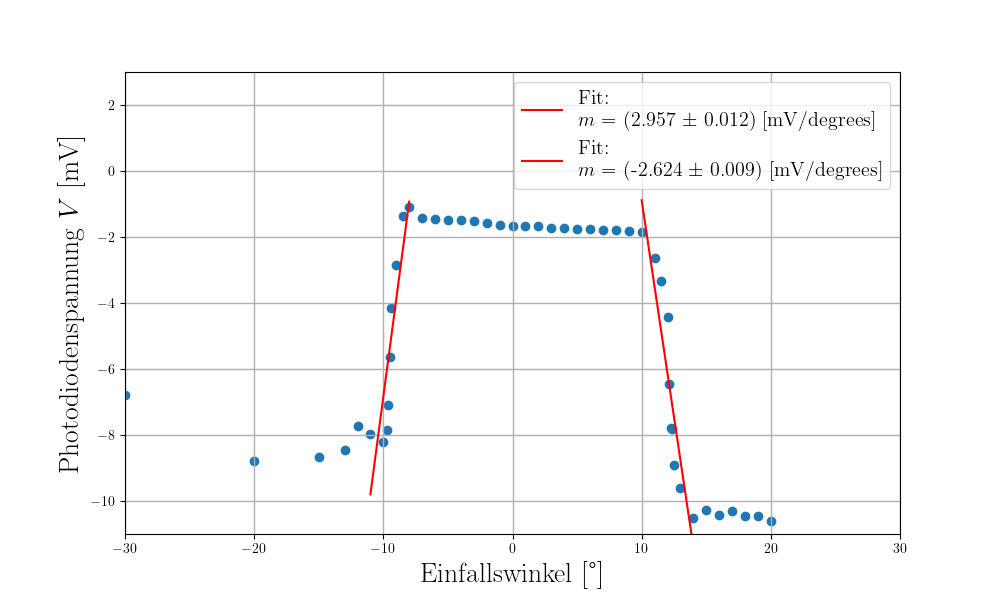
\includegraphics{Justierung.png}}
   \caption{Gemessene Abhängigkeit der Photodiodenspannung zur Einfallswinkel (blue Punkte) zusammen mit Linear-Fit der Flanken der Kurve (rote Linien).}
   \label{fig:justierung}
\end{figure}

Während der Durchführung dieses Versuchsteils, merken wir, dass der Laser nicht stabil ist, denn die Intensität des Lasers signifikant abnimmt zum Punkt wo keine Messungen nehmen werden können. Unser Betreuer kann erfolgreich das Fehler lösen. 

Um die Cut-on Winkeln aus diesem Diagramm zu ermitteln, passen wir einen letzten Fit an der Plateau der Kurve. Zunächst rechnen wir den Schnittstellen den Flankenfits mit diesem letzten Fit. Wir schätzen folgende Cut-On-Winkeln:
$$\vartheta_1 =  \SI{-8.18\pm 0.17}{\degree}$$ 
$$\vartheta_2 =  \SI{10.36\pm 0.21}{\degree}$$ 

Als zweite Schritt, messen wir die Abhängigkeit der Zählrate zur  angelegten Beschleunigungsspannung $U_B$ um die s.g. PMT-Kennlinie darzustellen. Während der Durchführung dieses zweiten Versuchsteils treten erneut Fehlern bei der Messungen, die aufgrund die Instabilität des Lasers erzeugen werden. Der fehlerhafte Verhältnis des Lasers kann deutlich in Fig. \ref{fig:fehler} beobachtet werde. In dieser Diagramm sind unser Messungen zu sehen, welche signifikant von die Erwartungen abweichen. Die Problemen beim Laser sind zu komplex, und das Gerät kann nicht schnell genug repariert werden, damit wir weitere Messungen nehmen können. Auf diesen Grund, bekommen wir alten Messwerte vom unseren Betreue um die Auswertung des Versuch durchzuführen.  

\begin{figure}[htbp]
    \centering
    % First row
    \begin{subfigure}{0.45\textwidth}
        \centering
        \resizebox{1.0\textwidth}{!}{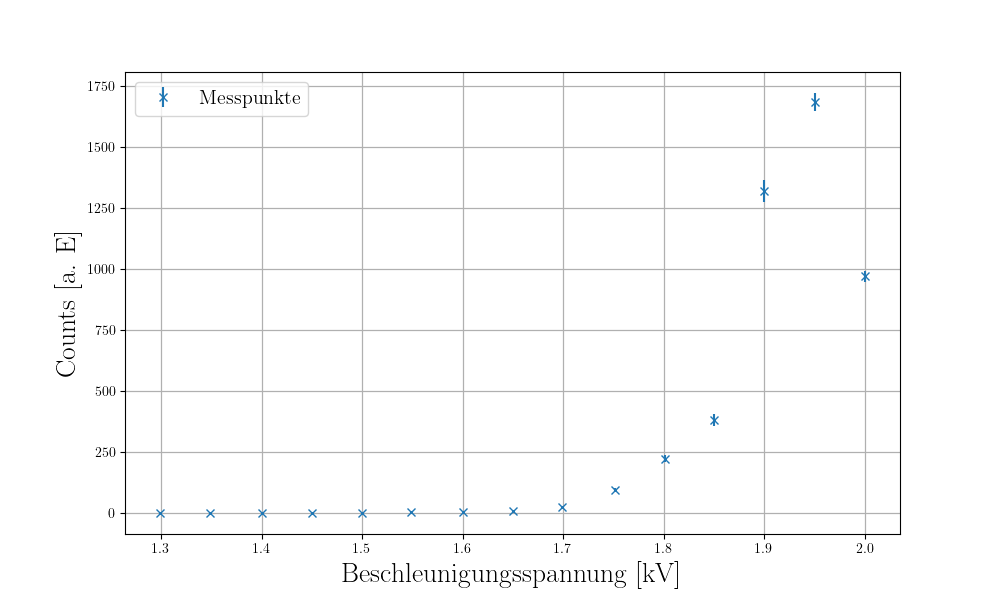
\includegraphics{PMT_Kennlinie_fail.png}}
        \caption{}
        \label{fig:fehler}
    \end{subfigure}
    \hfill
    \begin{subfigure}{0.45\textwidth}
        \centering
        \resizebox{1.0\textwidth}{!}{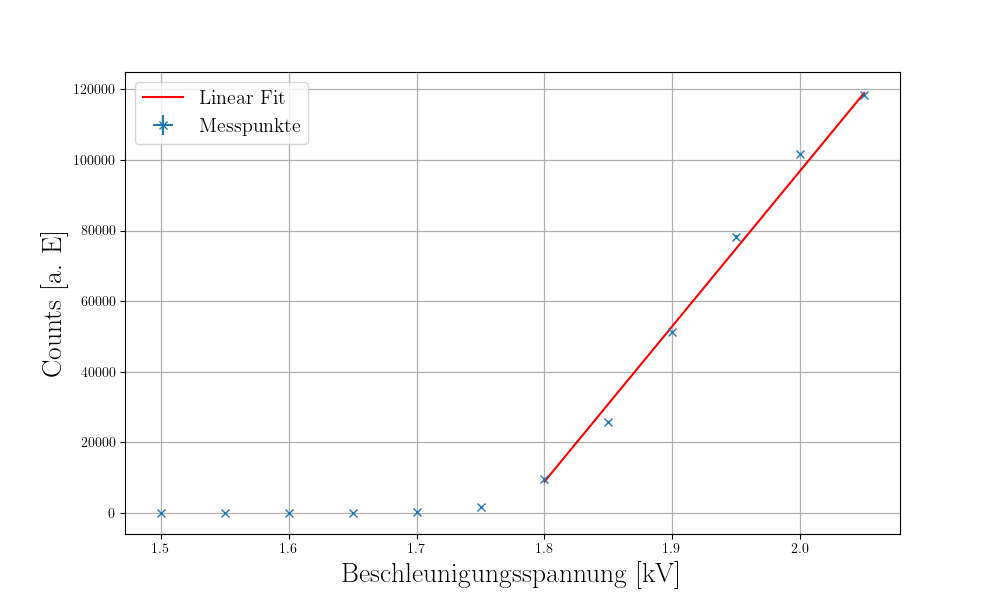
\includegraphics{PMT_Kennlinie.png}}
        \caption{}
        \label{fig:gegeben}
    \end{subfigure}
    % Second row copie first row
    \caption{PMT-Kennlinie. Abhängigkeit der Zählrate zur angelegten Beschleunigungspannung. a) Messreihe mit fehlerhaften Laser. b) Messreieh mit funktionsfähigen Laser (alte Messwerten vom Betreuer erhalten).}
    \label{fig:PMT_Kennlinie}
\end{figure}

In Fig. \ref{fig:gegeben} wird die PMT-Kennlinie des verwendetes Raman-Filter dargestellt. Aus diesem Diagramm können wir merken, dass im Bereich \num{1.8}$-$\SI{2.0}{\kilo\volt} die Zählrate ein linear Verhältnis zur $U_B$ zeigt. Um sinnvolle Messungen zu nehmen muss das Signal zu Dunkelstrom Verhältnis maximiert werden. Daher können wir ein Spannung $U_B =$ \SI{2.0}{\kilo\volt} als eine gute Wahl angeben.  

\section{Raman-Spektrum}
In diesen Versuchsteil untersuchen wir die Raman-Spektrum von normales- , para-Wasserstoff, Deuterium, Sauerstoff und Stickstoff. Zu jeden Messreihe gehört ein gemessenen Untergrundspektrum welche vom Spektrum abgezogen werden muss, um die Zählrate der ramngestreuten Photonen zu isolieren. 

\subsection{Rotationsspektrum von Deuterium}
Aus dem gemessenen Deuterium-Spektrum, Fig. \ref{fig:Deuterium}, können wir vier Raman-Linien beobachten. Um die gefundene Linien benenne zu können, müssen wir zum erste die erwartete Wellenlängenummer der Linien bestimmt werden.

Die Bestimmung der erwartete der Position der Raman-Linien wird mit der Literaturwerten der Masse von Deuterium und dem Atomabstand eines Deuteriummoleküls $D_2$ durchgeführt:
$$m_{D} =\SI{2.01588}{\atomicmassunit}$$
$$r_{D_2} = \SI{74}{\pm}.$$
Diese Werte setzen wir an der Gleichung
\begin{equation}
\label{eq:Rot_const}
B = \frac{h}{8\pi^2 c \mu r^2}
\end{equation}
um die erwartete Rotatioskonstante zu bestimmen. Hier $h$ entspricht die Planck'sche Konstant, $c$ die Lichtgeschwindigkeit und $\mu$ die reduzierte Masse:
\begin{equation}
\label{eq:redu_mass}
\mu = \dfrac{m_1\cdot m_2}{m_1 + m_2}.
\end{equation}
Da wir mit homogenen Moleküle arbeiten, gilt $m_1 = m_2$ und Gl. \ref{eq:redu_mass} vereinfacht sich:
\begin{equation}
\mu = \dfrac{1}{2} m.
\end{equation}
Wir finden: 
$$B_{lit}^{D_2} = \SI{30.57}{cm^{-1}}.$$
Die Wellenlängenummer der Rotationsanregungen wird durch
\begin{equation}
\label{eq:nu_rot,j} 
\bar{\nu}_{rot,J} = B(4J+6)
\end{equation}
gegeben. Und die Wellenlängenummer der Raman-Linie kann durch
\begin{equation}
\bar{\nu}_{J\to J+2} = \bar{\nu}_{Laser}\pm \bar{\nu}_{rot,J}
\end{equation}
ermittelt werden. In unser Experiment gilt:
$$\bar{\nu}_{Laser} = \SI{18691.59}{\centi\meter^{-1}}$$

Um die Position der gemessenen Raman-Linien quantitative betrachten zu können, passen wir eine Voigt-Distribution an der einzelne erkennbare Peaks an und als Fit-Funktion wird die Summe der einzelne angepasste Voigt-Profile gegeben. Die Voigt-Distributoin ist durch die Faltung einer Gauß- und einer Breit-Wigner Distribution definiert. Die Messwerte und die Fit-Funktion werden in Fig. \ref{fig:Deuterium} dargestellt.

Durch Vergleich der gemessenen und erwarteten Position der Linien, können wir die gemessenen Raman-Linien als die erste 4 Rotationsanregungen erkennen. Die gefundene und erwartete Werten werden in Tab. \ref{tab:D2} zusammengefasst und vergleicht. 

\begin{figure}[htbp]
	\centering
   \resizebox{.8\textwidth}{!}{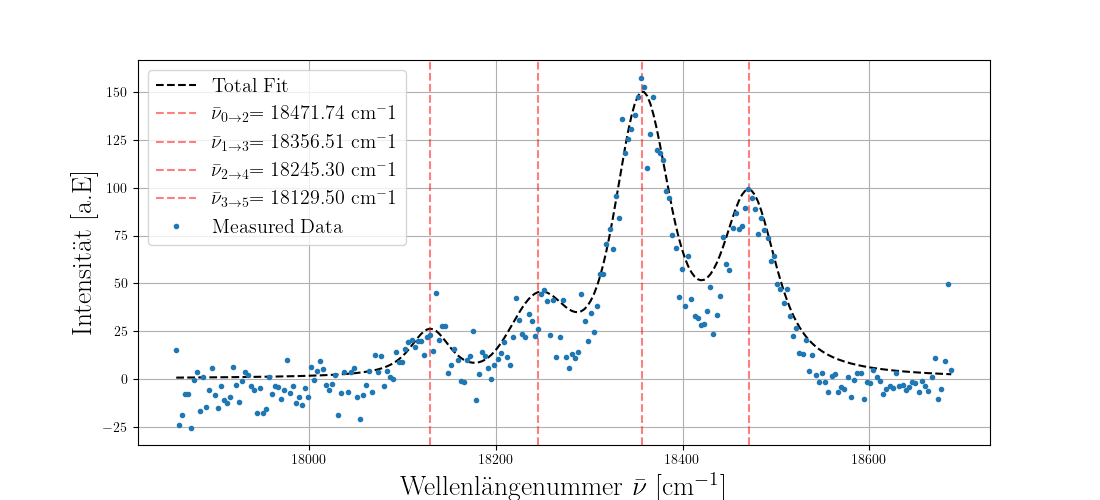
\includegraphics{D2_spektrum}}
   \caption{\small Raman-spectrum von Deuterium. Gemessenen Spektrum eine Deuterium Probe nach Untergrundabzug (blaue Punkte) mit Fit-Funktion, welche aus der Summe einzelnen Voigt-Fits besteht (schwarze Linie). Die gefundenen Raman-Linien sind durch gestrichelte rote Linien markiert.}
   \label{fig:Deuterium}
\end{figure}

\begin{table}[!htbp]
 \begin{center}
  \caption{\small Wellenlängenummer der Raman-Linien von $D_2$. Vergleich von erwartete und gemessene Werte.}
   \renewcommand{\arraystretch}{1.3} % Adjust 1.5 as needed
  \label{tab:D2}
  \begin{tabular}{|c|c|c|c|}
  \hline
\multirow{2}{*}{$J$}& \multicolumn{2}{c|}{$\bar{\nu}_{J\to J+2}$ [$\unit{cm^{-1}}$]} &  \multirow{2}{*}{ Abweichung $\sigma$} \\ \cline{2-3} % Horizontal line underthe multicolumn
 					 & gemessen & erwartet &    			\\ 
  \hline
	\hline 
0 & 18471.7	$\pm$ 1.1	& 18507.17	& 33.4 \\
1 & 18356.5	$\pm$ 0.9	& 18385.88	& 31.3 \\
2 & 18245	$\pm$ 3	& 18263.60	& 6.5	 \\
3 & 18129	$\pm$ 4		& 18141.32	& 3.22 \\
	\hline
  \end{tabular}
  \renewcommand{\arraystretch}{1} 

 \end{center}
\end{table}

Durch Bestimmung des Abstandes zwischen der Peaks können wir die Rotationskonstante von Deuterium bestimmen indem wir Gl. \ref{eq:nu_rot,j} verwenden. Durch dieser Art und Weise können wir 3 Werte für $B$ berechnen. Als Endergebnisse werden den Mittelwert und der zugehörige  Standardabweichung verwendet: 
$$B_{exp}^{D_2} = \SI{28.5\pm 0.5}{cm^{-1}}.$$
Wir beobachten eine signifikante Abweichung zum erwartete Wert:
$$\sigma_{B^D_2} = 4.01$$ 
 
Durch Umstellen von Gl. \ref{eq:redu_mass} können wir die reduzierte Masse $\mu$ abschätzen:
$$\mu_{exp}^{D_2} = \SI{1.079\pm 0.019}{\atomicmassunit}.$$
Dieser Wert zeigt, ebenfalls, eine signifikante Abweichung zur erwartete Wert $\mu_{lit} = \dfrac{1}{2}m_D$:
$$\sigma_{\mu^D_2} = 3.74.$$
Die große Abweichungen werden später ausführlich besprechen. 

\subsection{Rotationsspektrum von ortho- und para-Wasserstoff}
Zunächst, führen wir ein ähnliches Analyse wie bei Deuterium mit dem gemessenen Spektrum von ortho- und para-Wasserstoff durch.

Für die Bestimmung der erwartete Rotationskonstante und Wellenlängenummer der Raman-Linien verwenden wir folgende Werte für der Abstand von $H_2$ und Masse von $H$:

$$m_{H} =\SI{1.00794}{\atomicmassunit}$$
$$r_{H_2} = \SI{74}{\pm}.$$
Durch Einsetzen dieser Werte in Gl. \ref{eq:Rot_const} finden wir:
$$B_{lit}^{H_2} = \SI{61.0841}{cm^{-1}} $$

Analog wie bei letzten Abschnitt, passen wir ein Voigt-Distribution an jeder erkennbare Peak an und bilden die Fit-Fuktion aus die Summe der einzelne Voigt-Fits. Als Wellelängenummer wird die Position der Maxima der Distribution und der zugehörige Fehler angegeben. Das gemessene Spektrum von normal-$H_2$ zusammen mit der Fit-Funktion wird in Fig. \ref{fig:normal_H2} geplottet. Während das Spektrum der para-$H_2$ Probe wird in Fig. \ref{fig:para_H2} dargestellt. Mithilfe dieses letzten Diagramm stellen wir fest, dass die Untergrundmessung der para-$H_2$ Probe nicht erfolgreich war, denn nachdem der Untergrundabzug durchgeführt wird, beobachten wir eine Verschiebung des Spektrums um c.a 43 a.E in der y-Achse. 

Durch Vergleich der erwartete und gemessene Wellenlängenummer der Raman-Spektrum von Wasserstoff können wir die gefundene Peaks als die erste Rotationsanregungen erkennen. Die gemessene und erwartete Wellenlängernummer der Raman-Linien werden in Tab. \ref{tab:H2} zusamengefasst und vergleicht. Zusätzlich, wird die Intensität der Raman-Linien in der selben Tabelle zusammengefasst um die Reinheit der para-Wasserstoff abzuschätzen. 


\begin{figure}[htbp]
	\centering
   \resizebox{1.0\textwidth}{!}{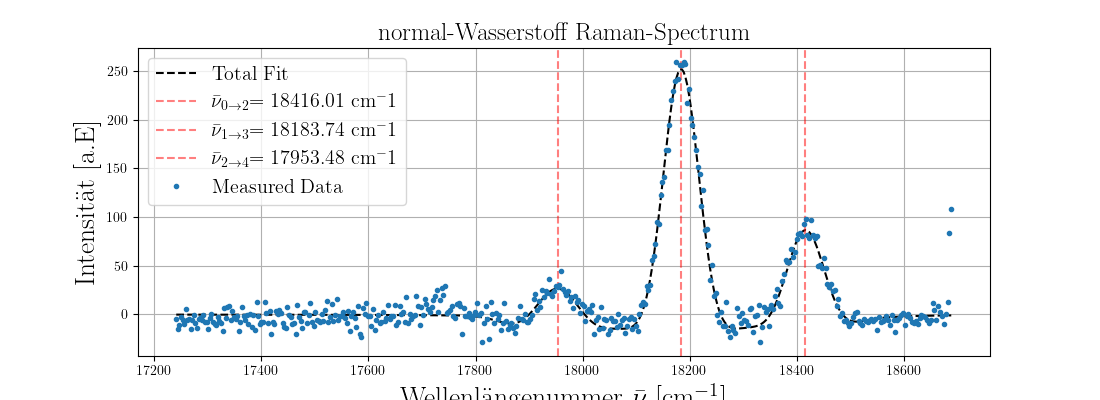
\includegraphics{H2_spektrum.png}}
   \caption{\small Raman-Spektrum von ortho-Wasserstoff. Gemessenen Spektrum eine normal-Wasserstoff Probe nach Untergrundabzug (blaue Punkte) mit Fit-Funktion (schwarze Linie). Die gefundene Raman-Linien sind durch gestrichtelte rote Linien markiert.}
   \label{fig:normal_H2}
\end{figure}

\begin{figure}[htbp]
	\centering
   \resizebox{1.0\textwidth}{!}{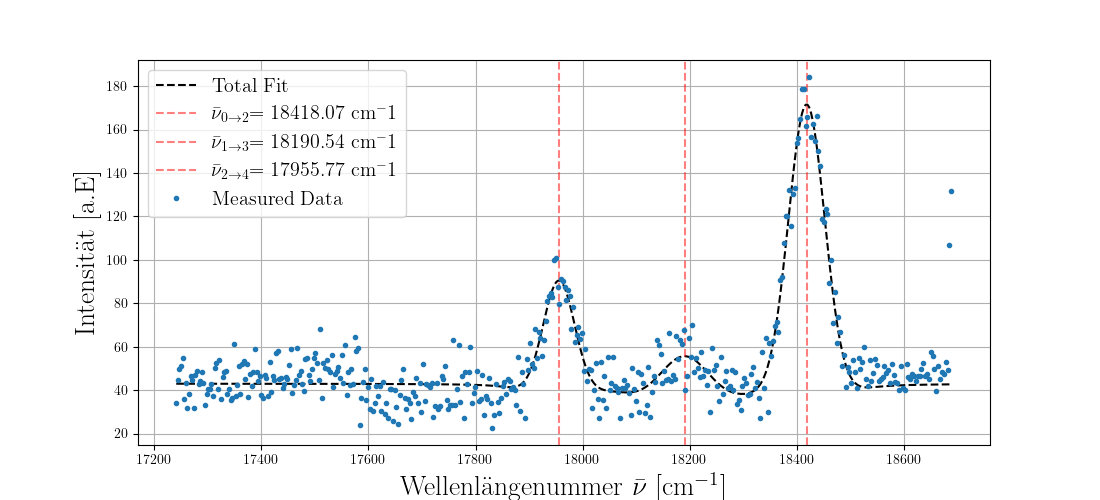
\includegraphics{paraH2_spektrum.png}}
   \caption{\small Raman-Spektrum von para-Wasserstoff. Gemessenen Spektrum eine normal-Wasserstoff Probe nach Untergrundabzug (blaue Punkte) mit Fit-Funktion (schwarze Linie). Die gefundene Raman-Linien sind durch gestrichtelte rote Linien markiert.}
   \label{fig:para_H2}
\end{figure}

Als erwarte, können wir sehen wie der Raman-Linie der ungeraden Vibrationsquanten in der para-$H_2$ Spektrum unterdrückt werden, Fig. \ref{fig:para_H2}, da diese zur ortho-Wasserstoff gehören. Wir erinnern uns, dass die beide Wasserstoffisomeren Spin 0 (para) und 1 (ortho) besitzen, und daher nur gerade oder ungerade Zustände erlaubt sind, aber nicht beiden. Die kleine, aber endliche Intensität der zweite Rotationsanregung, $I_{\nu  = 1 \to 3}$, besagt, dass die para-Wasserstoff Probe noch eine endliche Anzahl an ortho-$H_2$ besitzt. Durch Berechnung der Verhältnis zwischen die Intensität der erste $I_{\nu  = 0 \to 2}$ und zweite $I_{\nu  = 1 \to 3}$ Raman-Linien, können wir finden, dass in der para-$H_2$ Probe aus 1 Teil ortho- und 25 Teile para-Wasserstoff entsteht (1:25). Daher die Probe besteht aus c.a $96.2\%$ para-Wasserstoff und die Reinheit dieser kann als hoch beurteilt werden. Wird der Verhältnis der beide Intensitäten mit der Fitparameter der normal-Wasserstoff, so finden wir, dass die Probe ein Verhältnis 3:1 beschreibt, was mit der Literatur in klang liegt.  

\begin{table}[!htbp]
 \begin{center}
  \caption{\small Wellenlängenummer der Raman-Linien von $H_2$. Vergleich von erwartete und gemessene Werte einer para- und Normal-Wasserstoffprobe.}
  \label{tab:H2}
  % Increase the row height
  \renewcommand{\arraystretch}{1.3} % Adjust 1.5 as needed
  \begin{tabular}{|c|c|c|c|c|c|c|c|}
  \hline
\multirow{2}{*}{$J$}&\multicolumn{2}{c|}{Intensität [a.E]}& \multicolumn{3}{c|}{$\bar{\nu}_{J\to J+2}$ [$\unit{cm^{-1}}$]} & \multicolumn{2}{c|}{ Abweichung $\sigma$} \\ \cline{2-8} % Horizontal line under the multicolumn
 					 &$H_2^{norm.}$	&	$H_2^{para}$ & gem. $H_2^{norm.}$ & gem. $H_2^{para}$& erwartet &  $H_2^{norm.}$	&	$H_2^{para}$\\ 
  \hline
	\hline 
0 &	$\num{5211\pm450}$ 	&	$\num{10035\pm577}$	&	$\num{18416	\pm 1}$	& $\num{18418.1\pm 1}$	& 18325.08	& 91.8	& 116.12 \\ 
1 & 	$\num{16699\pm395}$	&	$\num{448\pm348}$	&	$\num{18183.7\pm0.4}$& $\num{18191\pm6}$	& 18080.75	& 279.12	& 18.78 \\ 
3 &	$\num{627\pm237}$	&	$\num{2926\pm333}$	&	$\num{17953\pm2}$	& $\num{17956\pm2}$	& 17836.41	& 53.59	& 76.24\\ 
	\hline
  \end{tabular}
  % Reset the row height to default
  \renewcommand{\arraystretch}{1}
 \end{center}
\end{table}

Aus der Tabelle können wir lesen, dass erneut signifikanten Abweichungen zwischen die erwartete und gemessene Werte bei beiden Messreihen, bzw. normal- und para-$H_2$, vorkommen.  

Durch bestimmen der Abstand zwischen der gemessene Raman-Linien lassen sich zwei Werten für die Rotationskonstante und zwei Werte für die reduzierte Masse, welche wir in Tab. \ref{tab:H2_B_mu} zusammenfassen und vergleichen. 

\begin{table}[!htbp]
 \begin{center}
  \caption{\small Wellenlängenummer der Raman-Linien von $H_2$. Vergleich von erwartete und gemessene Werte einer para- und Normal-Wasserstoffprobe.}
  \label{tab:H2_B_mu}
  % Increase the row height
  \renewcommand{\arraystretch}{1.3} % Adjust 1.5 as needed
  \begin{tabular}{|c|c|c|c|c|c|}
  \hline

\multirow{2}{*}{Größe}&\multicolumn{3}{c|}{Wert}& \multicolumn{2}{c|}{ Abweichung $\sigma$} \\ \cline{2-6} % Horizontal line under the multicolumn
 					 &$H_2^{norm.}$	&	$H_2^{para}$ &  $H_2^{lit}$ &  $H_2^{norm.}$	&	$H_2^{para}$\\ 
  \hline
	\hline 
B [$\unit{cm^{-1}}$] & $\num{57.8\pm0.3}$ & $\num{57.8\pm0.9}$ & 61.0841 & 13.03 & 3.64 \\
$\mu$ [$\unit{\atomicmassunit}$] & $\num{0.532\pm0.002}$& $\num{0.5\pm0.3}$&0.5004 &15.8 & 0.001\\
	\hline
  \end{tabular}
  % Reset the row height to default
  \renewcommand{\arraystretch}{1}
 \end{center}
\end{table}

Aus Tab. \ref{tab:H2_B_mu} lässt sich die Wirkungen der fehlerhafte Untergrundmessung für para-$H_2$ beobachten. Die Verschiebung in y-Achse hat die Genauigkeit der Fitparametern stark reduziert, im Vergleich zum normal-$H_2$. Für die Fits wurde es versuch die Verschiebung in y-Richtung miteinzubeziehen, trotzdem bleiben die Größe Unschärfe der Fitparameter. Aus diesem Grund kann sind die Abweichungen kleiner als bei normal-$H_2$, selbst wenn die Werte nicht signifikant näher am Literaturwert liegen. Die beobachtete signifikante Abweichungen werden später in der Diskussion behandeln. 

\subsection{Vibrationsanregung von Sauerstoff und Stickstoff}
In diese letzte Abschnitt betrachten wir die Vibrations-Raman Spektrum von Stickstoff und Sauerstoff. Aufgrund der höhere reduzierte Masse und Atomabstand beiden Moleküle, die Rotationskonstante ist deutlich kleine als die Rotationskonstante von Wasserstoff und die Auflösung unser Versuchsaufbau ist nicht hoch genug um die Rotationsstruktur aufzulösen. Trotzdem, da die Vibrationsanregungen eine höhere Energie besitzen, können wir die erste Schwingungsanregung auflösen und messen. 

Um die erwartete Wellenlängenummer abzuschätzen, berechnen wir die Vibrationskonstante für beide Moleküle mithilfe der Gleichung:
\begin{equation}
\omega_e = \omega \left( v + \dfrac{1}{2} \right),
\end{equation}
wo die Kreisfrequenz als 
\begin{equation}
\omega = \sqrt{\dfrac{\kappa}{\mu}} = \sqrt{\dfrac{E_{B}}{r^2\mu}}
\end{equation}


\end{document}
